\chapter{\tl{DCCA Optimizations}}
\en{Before the classification, we must optimize the DCCA network parameters, and find the ideal values and combinations. We do that for the different cases of the views. 

First of all, we train the DCCA networks on the raw data, meaning the 145 ROI values for the imaging view, and the 54 SNPs for the genetic view. After that, we take the MCA-transformed genetic data (10 genetic components), and pair them with the original imaging data, meaning the 145 ROI values. Finally, we experiment with the opposite combination, which is the OPNMF-transformed imaging data (30 imaging components) and pair them with the original genetic data, meaning the 54 SNPs. 

As mentioned in the previous chapter, the parameter combinations we explored affect the number and sizes of the hidden layers, the size of the output layer of the network, the learning rate, the regularization parameter and the batch size. The following results are after exhaustive search of the different parameter combinations. 

The metric we optimized for is the correlation between the two views, after being transformed by their respective DCCA network. Essentially we pass the data through their own trained network, transforming them and measuring how linearly correlated they have become. The total number of parameter combinations for each different case of the views is 288.

For each parameter, we plotted for the different values the correlation achieved by the worst combination of the parameter’s value with all the other possible parameters values, the average correlation, as well as the best correlation. Since the implementation of the DCCA network employed the correlation as a Loss function (assigned with a negative signum, in order to be able to be minimized), we used that as the metric directly. 

\section{\tl{Original data: 145 ROI (Imaging) + 54 SNPs (Genetic)}}

\begin{figure}[H]
    \centering
    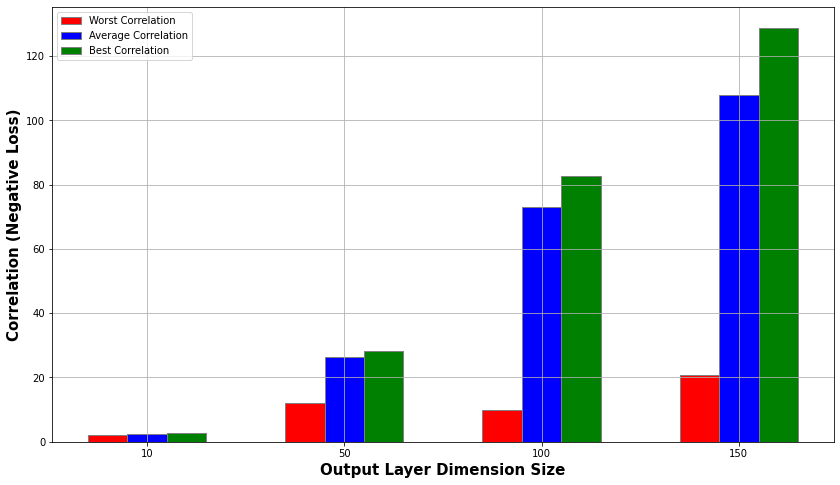
\includegraphics[width=\textwidth]{figures/DCCA_optimizations/Raw_Outdim.png}
    \caption{\en{Output Layer Dimension size vs Achieved Correlation}}
\end{figure}
\begin{figure}[H]
    \centering
    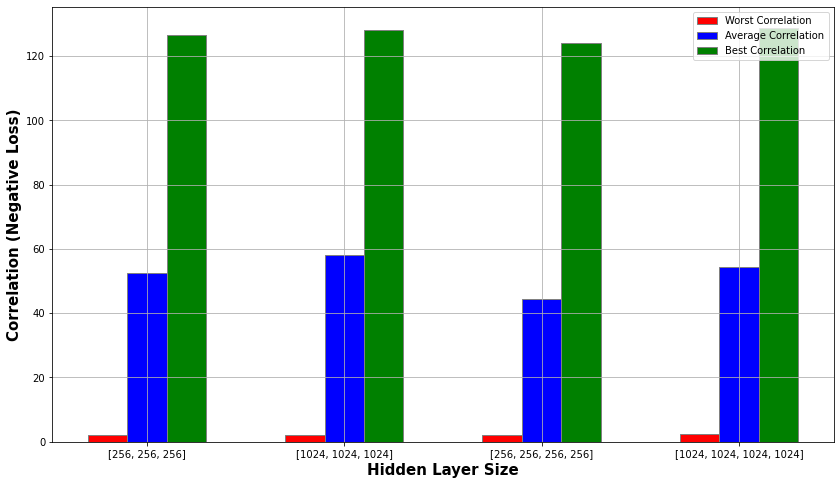
\includegraphics[width=\textwidth]{figures/DCCA_optimizations/Raw_Hidden.png}
    \caption{\en{Hidden Layer size vs Achieved Correlation}}
\end{figure}
\begin{figure}[H]
    \centering
    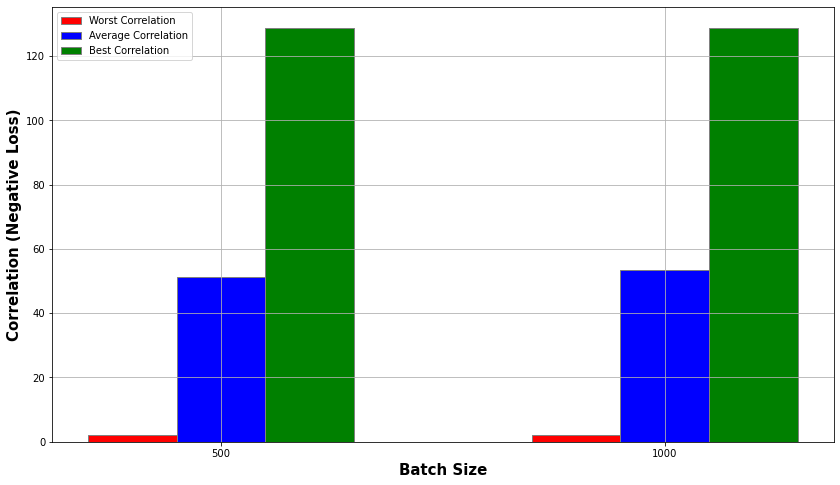
\includegraphics[width=\textwidth]{figures/DCCA_optimizations/Raw_Batch.png}
    \caption{\en{Batch size vs Achieved Correlation}}
\end{figure}
\begin{figure}[H]
    \centering
    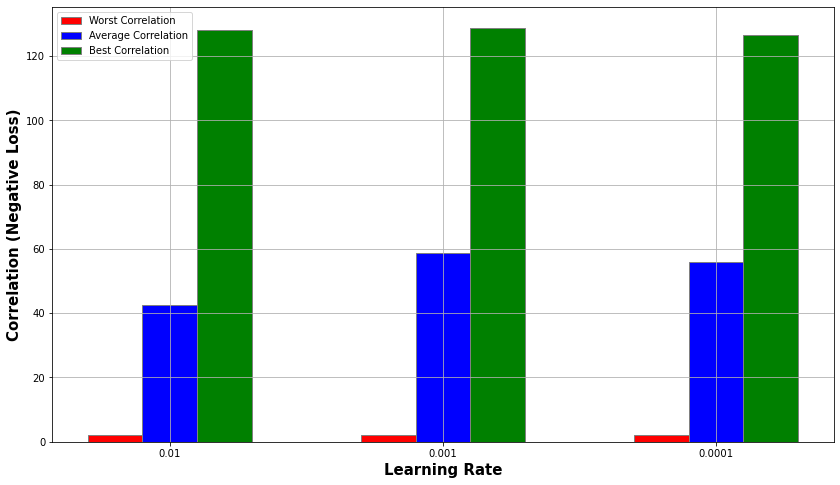
\includegraphics[width=\textwidth]{figures/DCCA_optimizations/Raw_Learning.png}
    \caption{\en{Learning Rate vs Achieved Correlation}}
\end{figure}
\begin{figure}[H]
    \centering
    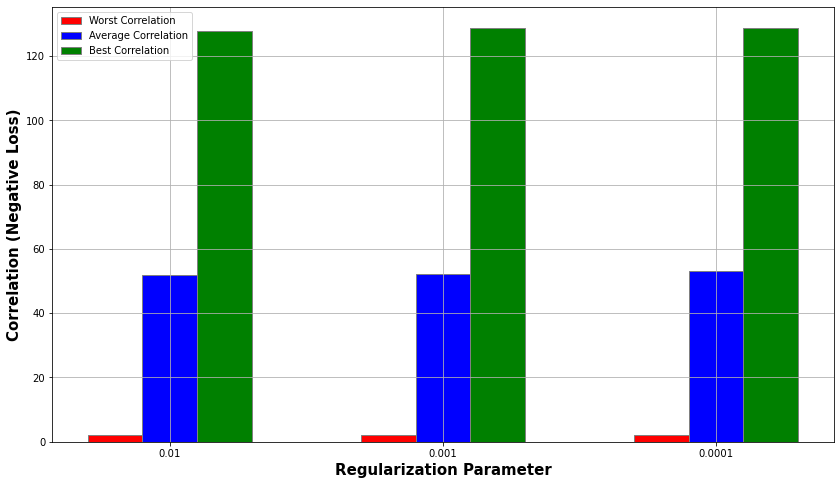
\includegraphics[width=\textwidth]{figures/DCCA_optimizations/Raw_Regularization.png}
    \caption{\en{Regularization Parameter vs Achieved Correlation}}
\end{figure}


Based on the above figures, it is clear that the more nodes the output layer has, the better the correlation of the transformed data is, not only on the best case, but on average as well as on the worst case. 

Furthermore, it is clear that the hidden layer size and number have little effect on the output correlation, since not only the best, but also the average and the worst cases, the correlation numbers seem to be the same. It can be noted that more hidden layers and more nodes per hidden layer do seem to be achieving better results, but the difference is minor.  

As for the batch size parameters, in our experiments the results stay basically identical; the only change being noticed in terms of training time, since the lower the batch size, the more time the model takes per epoch to run through the dataset, hence more training time for the same number of epochs. 

The same effect can be noticed with the Learning Rate, since the best case is more or less achieving the same results, however here we can observe that the average case benefits from a medium Learning Rate value of 0.001. 

Finally, the Regularization parameter follows the same logic, with its changing not making a substantial difference, and on all accounts the results being identical. 

To summarize the parameters' effects, we can create the following table:

\begin{figure}[H]
    \centering
    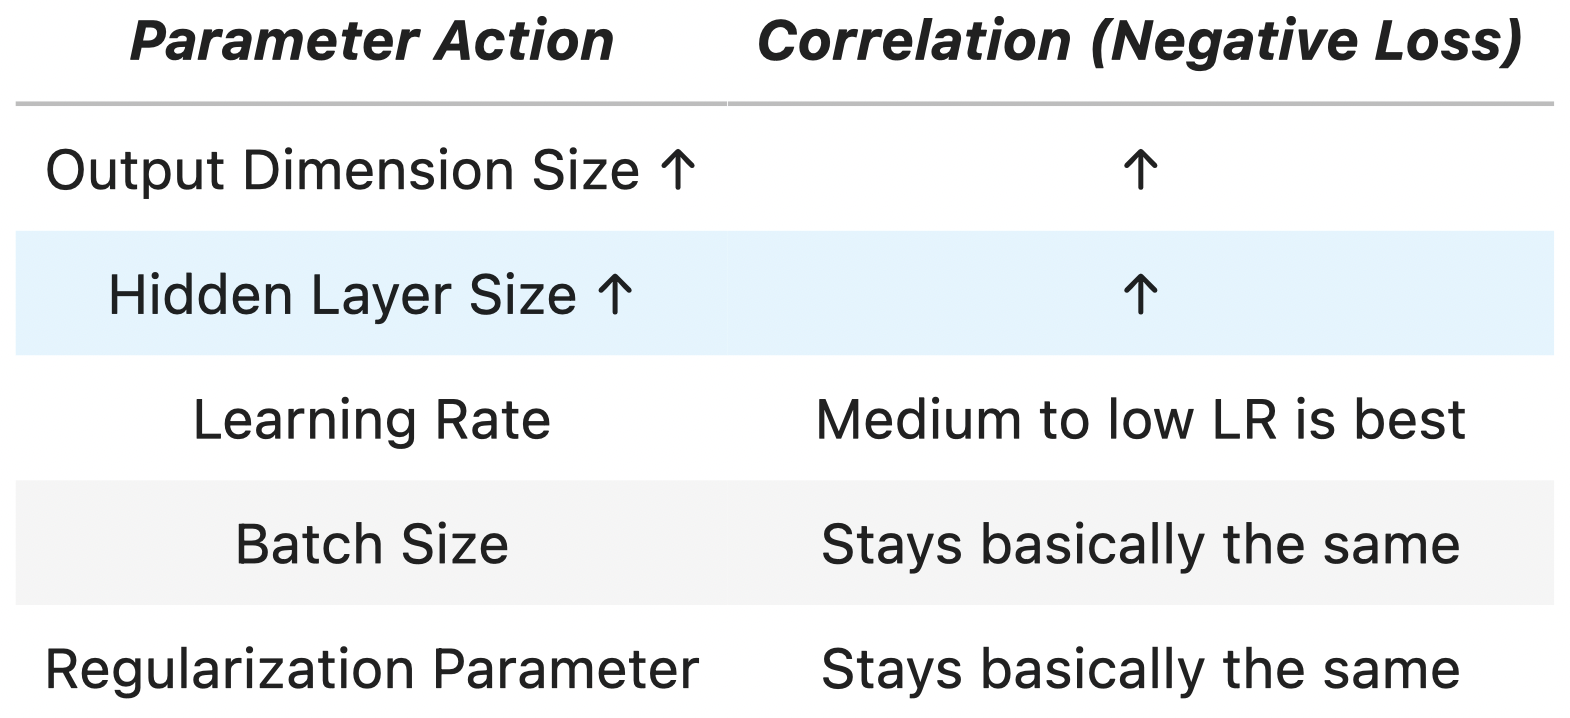
\includegraphics[width=0.7\textwidth]{figures/DCCA_optimizations/Raw_Conclusions.png}
    \caption{\en{Learned Conclusions from DCCA optimizations on 145 ROI (Imaging) and 54 SNPs (Genetic)}}
\end{figure}

\section{\tl{Transformed Genetic data: 145 ROI (Imaging) + 10 MCA components (Genetic)}}
\begin{figure}[H]
    \centering
    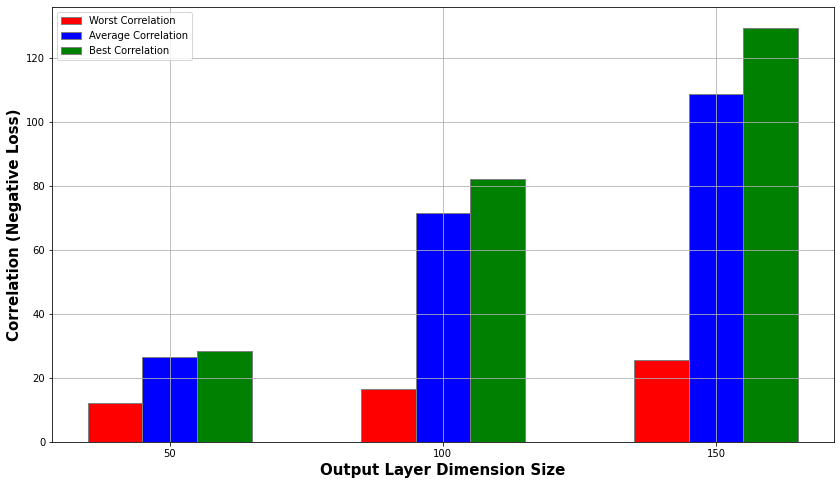
\includegraphics[width=\textwidth]{figures/DCCA_optimizations/MCA_Outdim.png}
    \caption{\en{Output Layer Dimension size vs Achieved Correlation}}
\end{figure}
\begin{figure}[H]
    \centering
    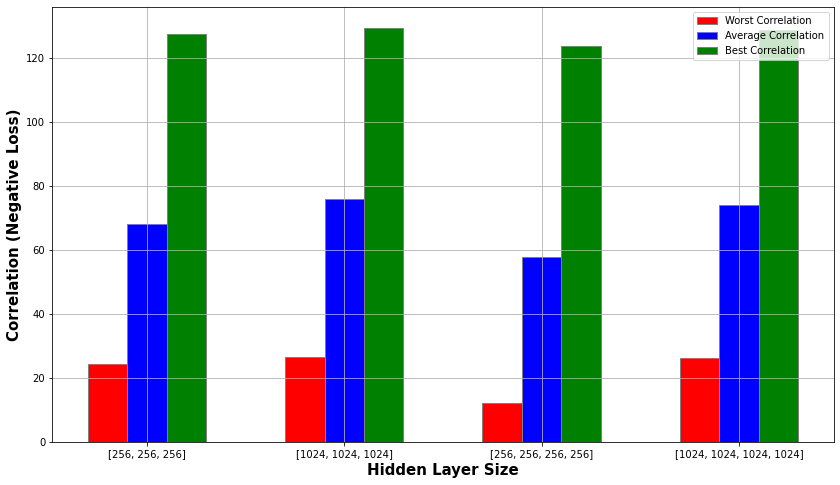
\includegraphics[width=\textwidth]{figures/DCCA_optimizations/MCA_Hidden.png}
    \caption{\en{Hidden Layer size vs Achieved Correlation}}
\end{figure}
\begin{figure}[H]
    \centering
    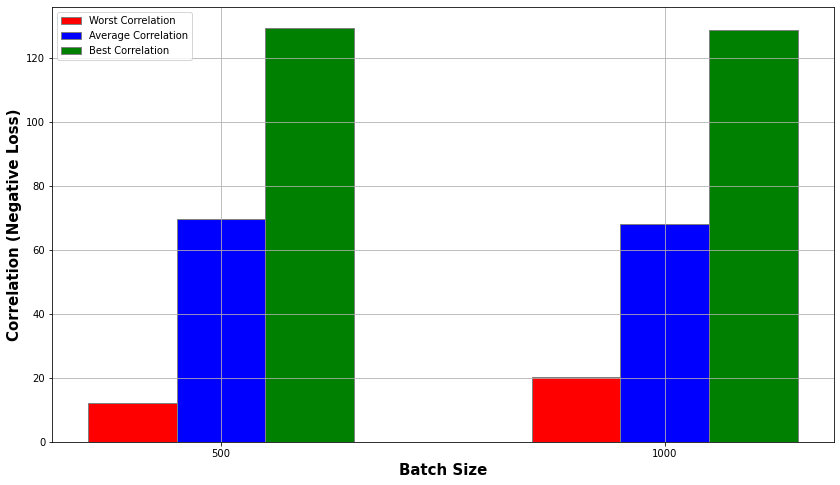
\includegraphics[width=\textwidth]{figures/DCCA_optimizations/MCA_Batch.png}
    \caption{\en{Batch size vs Achieved Correlation}}
\end{figure}
\begin{figure}[H]
    \centering
    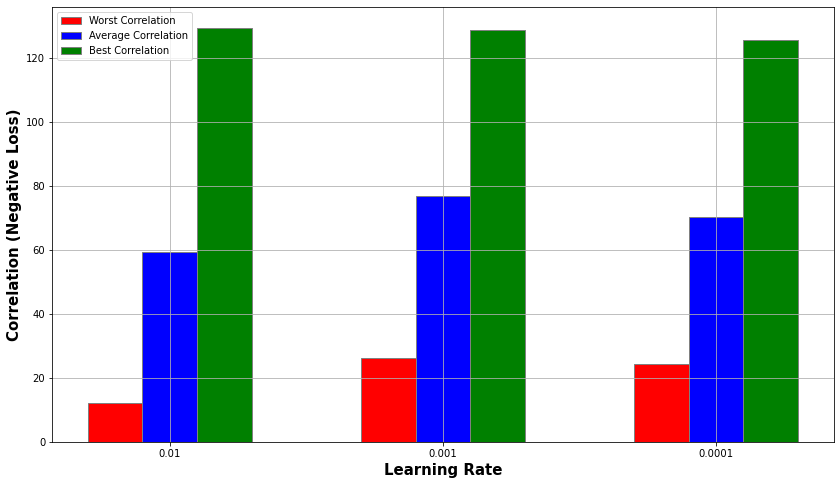
\includegraphics[width=\textwidth]{figures/DCCA_optimizations/MCA_Learning.png}
    \caption{\en{Learning Rate vs Achieved Correlation}}
\end{figure}
\begin{figure}[H]
    \centering
    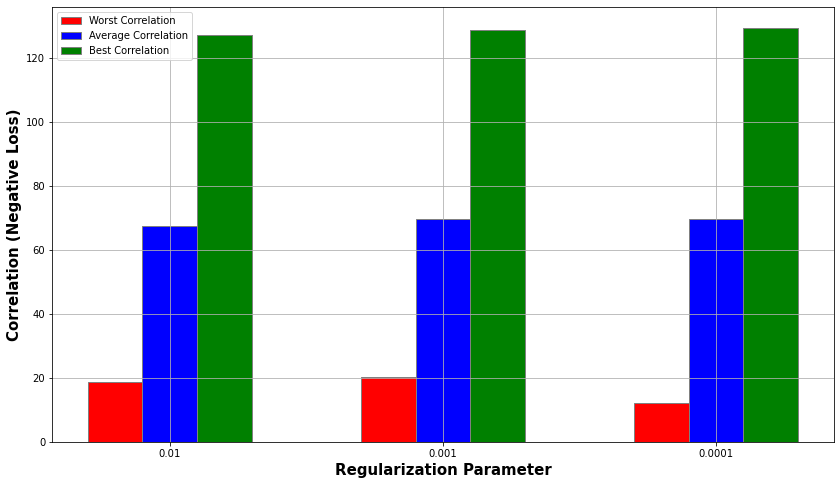
\includegraphics[width=\textwidth]{figures/DCCA_optimizations/MCA_Regularization.png}
    \caption{\en{Regularization Parameter vs Achieved Correlation}}
\end{figure}

As before, we notice the same patterns. Increasing the output layer size results in an increase in output correlation, hidden layer size and number of hidden layers seems to make a small difference, and for the rest of the parameters the effect seems to be negligible. We can sum up the parameter behaviour in the following table:
\begin{figure}[H]
    \centering
    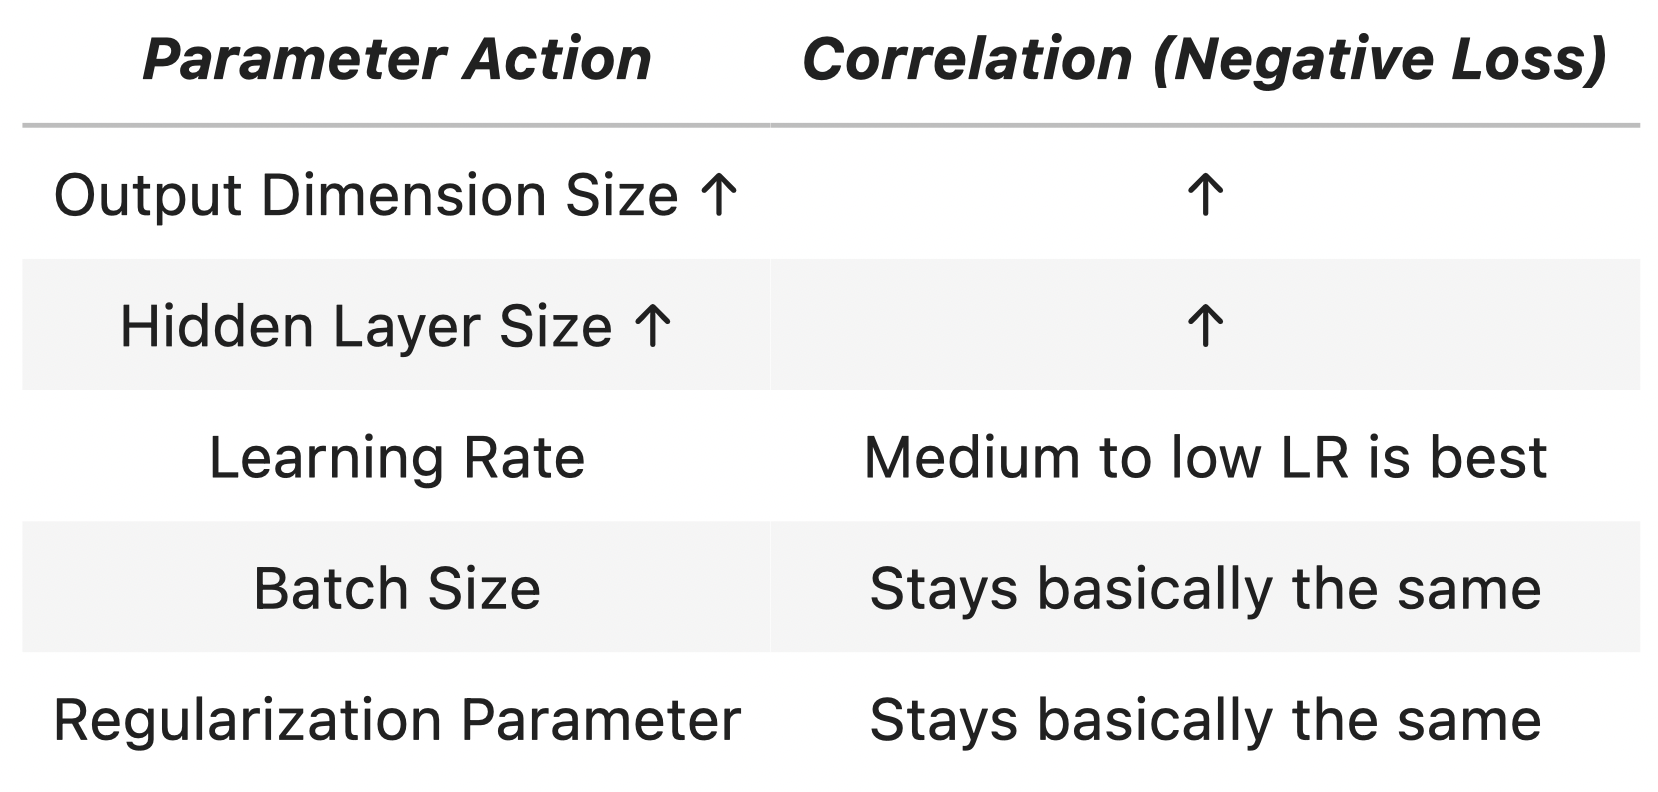
\includegraphics[width=0.7\textwidth]{figures/DCCA_optimizations/MCA_Conclusions.png}
    \caption{\en{Learned Conclusions from DCCA optimizations on 145 ROI (Imaging) and 10 MCA Genetic components}}
\end{figure}


\section{\tl{Transformed Imaging data: 30 OPNMF components (Imaging) + 54 SNPs (Genetic)}}

\begin{figure}[H]
    \centering
    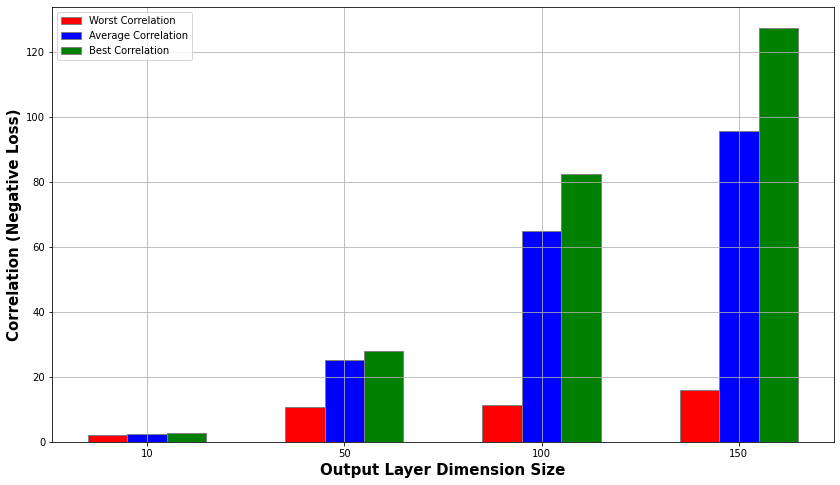
\includegraphics[width=\textwidth]{figures/DCCA_optimizations/NMF_Outdim.png}
    \caption{\en{Output Layer Dimension size vs Achieved Correlation}}
\end{figure}
\begin{figure}[H]
    \centering
    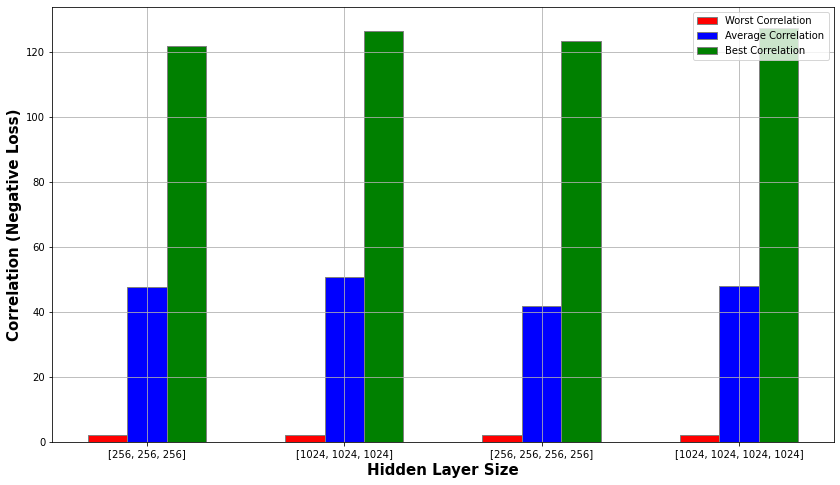
\includegraphics[width=\textwidth]{figures/DCCA_optimizations/NMF_Hidden.png}
    \caption{\en{Hidden Layer size vs Achieved Correlation}}
\end{figure}
\begin{figure}[H]
    \centering
    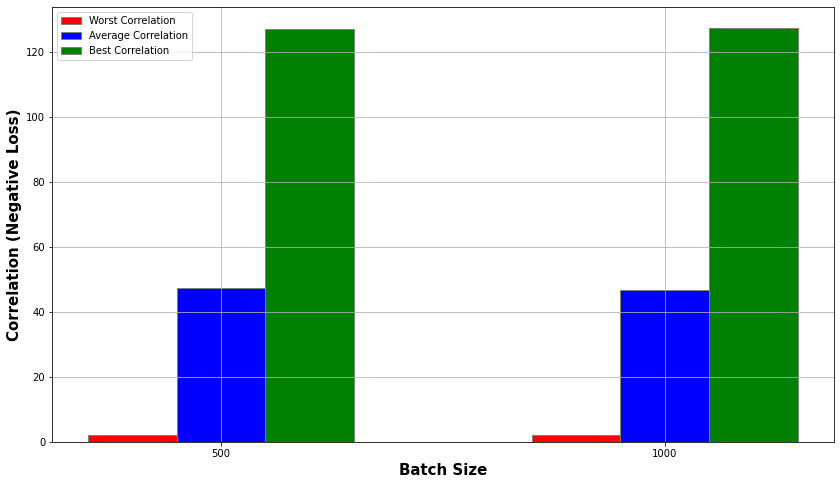
\includegraphics[width=\textwidth]{figures/DCCA_optimizations/NMF_Batch.png}
    \caption{\en{Batch size vs Achieved Correlation}}
\end{figure}
\begin{figure}[H]
    \centering
    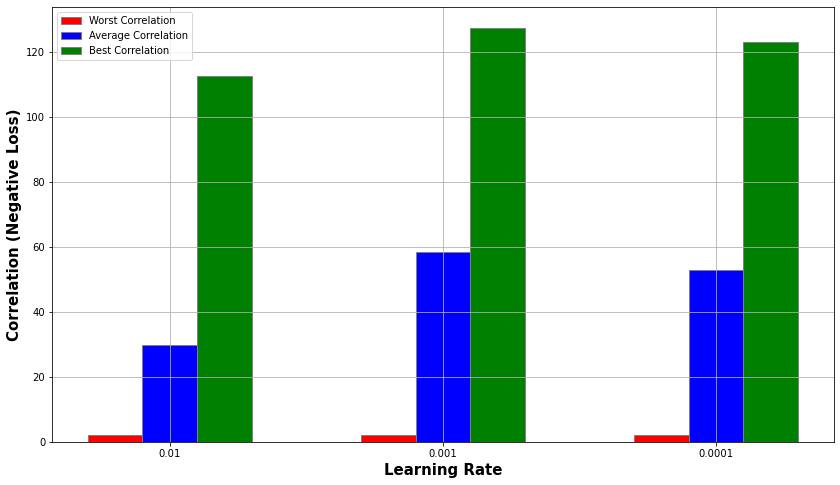
\includegraphics[width=\textwidth]{figures/DCCA_optimizations/NMF_Learning.png}
    \caption{\en{Learning Rate vs Achieved Correlation}}
\end{figure}
\begin{figure}[H]
    \centering
    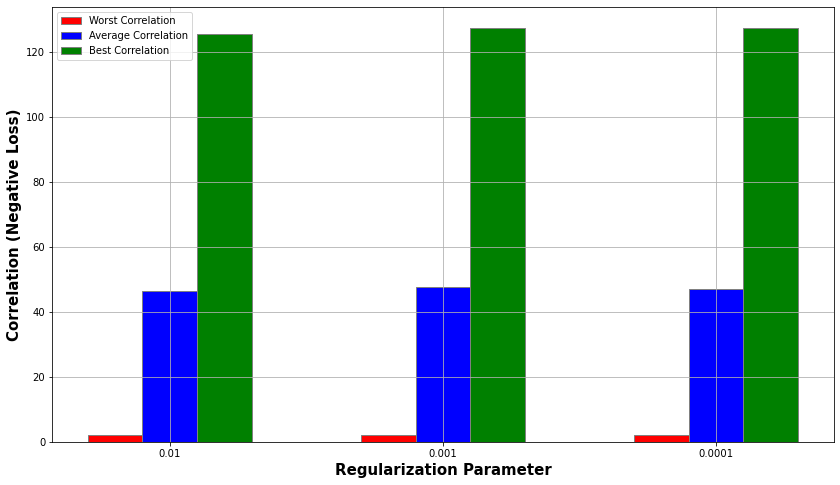
\includegraphics[width=\textwidth]{figures/DCCA_optimizations/NMF_Regularization.png}
    \caption{\en{Regularization Parameter vs Achieved Correlation}}
\end{figure}

Finally, in the case of the transformed through OPNMF imaging data combined with the raw genetic data, we can see that the parameter behaviour is again the same. Once again, output layer size increase correlates with better results, bigger hidden layer size, along with increasing the number of hidden layers improves the output correlation but only slightly, learning rate should be kept at a value of 0.001, and altering the other parameters has little to no effect.  

\begin{figure}[H]
    \centering
    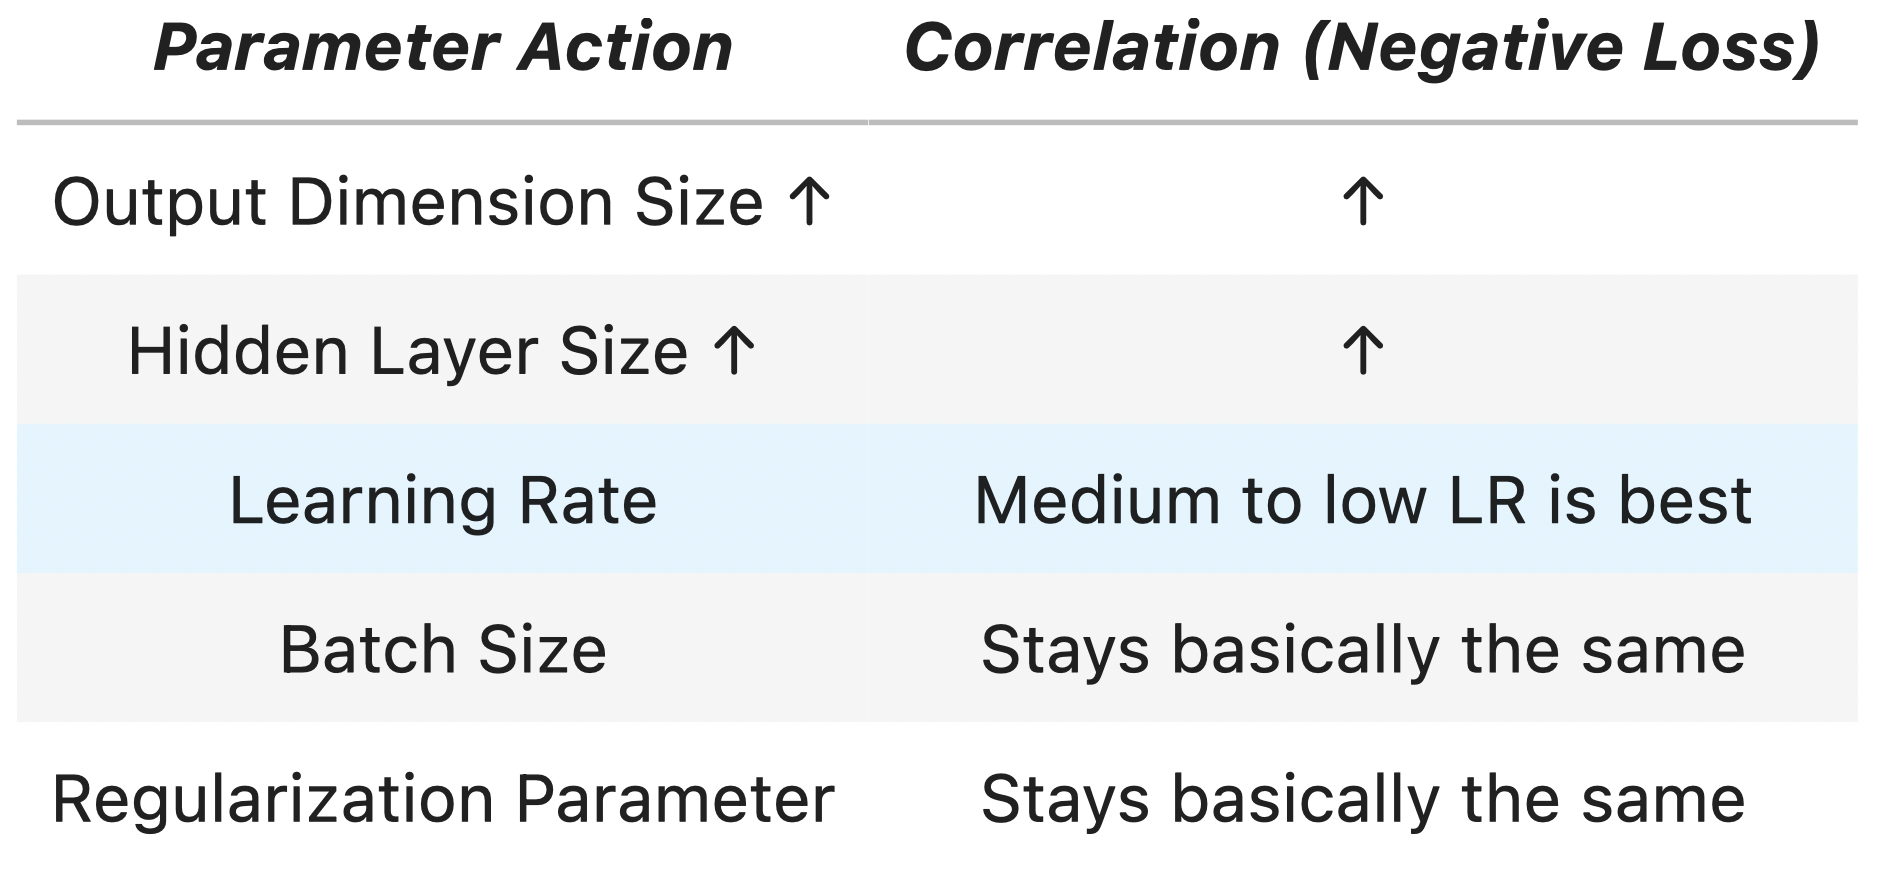
\includegraphics[width=0.7\textwidth]{figures/DCCA_optimizations/NMF_Conclusions.png}
    \caption{\en{Learned Conclusions from DCCA optimizations on 54 Imaging components and and 54 SNPs (Genetic)}}
\end{figure}
}